\documentclass[10pt,a4paper]{report}
\usepackage[margin=1.25in]{geometry}
\usepackage[pdftex]{graphicx}
\usepackage{subfigure}            % Multiple figures per float
\usepackage{placeins}             % Fix float loactions with \FloatBarrier
\usepackage{color}                % Color definitions for boxes
\usepackage{multirow}             % Multiple rows per cell in a table
\usepackage{verbatim}             % Long verbatim sections
\usepackage{titlesec}             % Easy modification the chapter format
\usepackage{fancyhdr}             % Easy modification of header and footer
\usepackage{hyperref}				% Custom hyperlinks
\usepackage{tikz}					% Figures and trees
\usetikzlibrary{arrows,shapes,positioning,shadows,trees}

\renewcommand{\arraystretch}{1.2} % Extra space in tables
\parindent0mm                     % New paragraphs start without indentation
\setlength{\parskip}{1em}         % And with a blank line in between

\tikzset{
  basic/.style  = {draw, text width=2.5cm, drop shadow, font=\sffamily, rectangle},
  root/.style   = {basic, rounded corners=2pt, thin, align=center,
                   fill=green!30},
  level 2/.style = {basic, rounded corners=6pt, thin,align=center, fill=green!60,
                   text width=10em},
  level 3/.style = {basic, thin, align=left, fill=blue!30, text width=8em},
  level 4/.style = {basic, thin, align=left, fill=blue!60, text width=8em},
  level 5/.style = {basic, thin, align=left, fill=gray!60, text width=10em}
}

% Redefine chapters to remove the "Chapter" word
\titleformat{\chapter}
  {\normalfont\LARGE\bfseries}{\thechapter}{1em}{}
\titlespacing*{\chapter}{0pt}{3.5ex plus 1ex minus .2ex}{2.3ex plus .2ex}

% Setup hyperlink format in document
\hypersetup{
    colorlinks=true, %set true if you want colored links
    linkcolor=blue,  %choose some color if you want links to stand out
    citecolor=blue,  %choose some color if you want lcitation to stand out
    filecolor=black, % etc...
    urlcolor=blue
}

% Define header and footer
\pagestyle{fancy}
\fancyhf{}
\lhead{C. Rosales, A. G\'{o}mez}
\rhead{REMORA User Guide}
\lfoot{REMORA User Guide}
\rfoot{\thepage}

% Define header and footer for first page in chapter
\fancypagestyle{plain}{
\fancyhf{}
\lhead{C. Rosales, A. G\'{o}mez}
\rhead{REMORA User Guide}
\lfoot{REMORA User Guide}
\rfoot{\thepage}
}

% Gray boxes for optional material
\definecolor{LightGrey}{gray}{.85}
\setlength{\fboxrule}{1pt}
\setlength{\fboxsep}{6pt}
\newcommand{\IntroBox}[1]{
  %\fcolorbox[rgb]{0,0,0}{0.95,0.95,0.95}{
    \fcolorbox{black}{LightGrey}{
    \begin{minipage}{0.94\linewidth}
      %\textbf{Introduction}
      #1
    \end{minipage}
  }
}




\begin{document}

\begin{titlepage}
\thispagestyle{empty}	%don't include number on cover
%\begin{flushleft}
%\begin{figure}
%\includegraphics[width=0.2\textwidth]{gplv3-127x51.png}
%\end{figure}
%\end{flushleft}
\verb+ +
\vspace{1em}
\begin{flushright}
\huge\bf REMORA v1.8\\
\rule{\textwidth}{4pt}
\large{\bf REsource MOnitoring for Remote Applications\\
Document Revision 1.0\\
\today}
\end{flushright}

\begin{figure}[ht!]
	\centering
	
\includegraphics[width=0.5\columnwidth]{logos/Remora-logo-600px.png}
\end{figure}

%Back of cover page (copyright)
\newpage
\thispagestyle{empty}
\begin{flushleft}
Antonio G\'omez-Iglesias, Carlos Rosales Fern\'andez \\
\verb+agomez@tacc.utexas.edu+, \verb+carlos@tacc.utexas.edu+\\
\vspace{0.5em}
High Performance Computing \\
Texas Advanced Computing Center\\
The University of Texas at Austin\\
\vspace{1cm}
Copyright 2017 The University of Texas at Austin.
\end{flushleft}
\newpage
\end{titlepage}

\begin{abstract}

REMORA is a modular tool to monitor runtime resource utilization in HPC environments. As of version 1.8 the suite contains code designed to test:

\begin{itemize}
\item Memory utilization in CPUs, Xeon Phi co-processors, and NVIDIA GPUs
\item CPU utilization
\item IO utilization for the Lustre and DVS file systems
\item NUMA properties
\item Network topology
\item Power consumption
\item CPU temperature
\end{itemize}

Throughout the text we have used text boxes to highlight important information. These boxes look like this:

\IntroBox{These gray boxes contain highlighted material for each section and chapter.}

Our intention is to create a simple runtime resource monitoring tool that provides both simple to understand high level information to the user, as well as detailed statistics for in-depth analysis. We welcome all feedback. Feedback that includes suggestions for improvement in the usability, reliability, and accuracy of this tool is particularly welcome. 

Version 1.8 is a new release that includes MPI support and improved visualization of the results.

REMORA is an open-source project. Funding to keep researchers working on REMORA depends on the value of this tool to the scientific community. We would appreciate if you could include the following citation in your scientific articles:

C. Rosales, A. G\'{o}mez-Iglesias, A. Predoehl. ``REMORA: a Resource Monitoring Tool for Everyone''. HUST2015 November 15-20, 2015, Austin, TX, USA. DOI: 10.1145/2834996.2834999 \cite{remora}

\end{abstract}

\tableofcontents

\chapter{Installation}
REMORA is simple to install. In order to use all of its features you will need GNU Make and a C compiler. If testing the Xeon Phi you will also need a compiler with support for compilation of native code for the Xeon Phi - currently limited to Intel 13+ compilers.

First of all obtain the latest version tarball, currently remora-1.8.tar.gz \footnote{\href{https://github.com/TACC/remora/archive/v1.8.tar.gz}{https://github.com/TACC/remora/archive/v1.8.tar.gz}}, and expand it in a convenient location in your system:

\begin{verbatim}
    tar xzvf ./remora-1.8.tar.gz
\end{verbatim}

Alternatively clone the git repository with the latest development version (not recommended):

\begin{verbatim}
    git clone https://github.com/TACC/remora
\end{verbatim}

This will create a top level directory called \verb+remora+, with subdirectories \verb+/scripts+, \verb+/docs+ and \verb+extra+. Change directory to the top level of remora and edit \verb+install.sh+ to reflect your choice of installation directory, build type, and modules configuration. The variables to modify are:

\begin{table}[h]
\centering
\label{tab:env}
\begin{tabular}{|l|l|l|}
\hline
\bf{Variable}	& \bf{Description}                          & \bf{Default}\\\hline
REMORA\_DIR     & Absolute path to installation directory   & . \\\hline
PHI\_BUILD      & Enable (1) or disable (0) Xeon Phi build  & 0 \\\hline
\end{tabular}
\end{table}

The modules are configured in the \verb+src\config\modules+ file. Simply remove any modules that you don't want to be available in your system. Also, you can create your own modules and add them into this file (see Section \ref{expand-remora} for more information about how to expand REMORA's functionality).

Once these variables are set the tool can be installed by using:

\begin{verbatim}
    ./install.sh
\end{verbatim}

The executable tests will be placed in the \verb+remora/bin+ directory unless the \verb+REMORA_DIR=/install/dir/location/+ has been modified at the top of the installation script. An installation path can also be specified on the command line:

\begin{verbatim}
    REMORA_INSTALL_PREFIX=</install/dir/location> ./install.sh
\end{verbatim}

\FloatBarrier
\chapter{Using REMORA}

\section{Collecting Data}
After installing remora please make sure the remora \verb+bin+ directory is in your \verb+PATH+ and the remora \verb+lib+ directory is in your \verb|LD_LIBRARY_PATH|. You should also define the environmental variable \verb+REMORA_BIN+ tot eh remora \verb+bin+ directory. If you are using a system wide installation this has probably been done by your system administrator. If you are doing it yourself the set of commands you need for an installation under \verb+/home/carlos/remora+ is the following:

\begin{verbatim}
	export REMORA_BIN=/home/carlos/remora/bin
	export PATH=$PATH:$REMORA_BIN
	export LD_LIBRARY_PATH=$LD_LIBRARY_PATH:/home/carlos/remora/lib
\end{verbatim}

You may want to add these to your startup files to ensure REMORA is available every time you login. Once this setup has been done running remora is extremely simple.

For a serial job:

\begin{verbatim}
	remora ./myexe [myexe_arguments]
\end{verbatim} 

For a parallel job (assuming \verb+mpirun+ is your parallel launcher, change for mpiexec.hydra, ibrun or other as needed):

\begin{verbatim}
	remora mpirun [mpirun_options] ./myexe [myexe_arguments]
\end{verbatim} 

The code will run as normal, and at the end a directory called \verb+remora_<jobid>+ where \verb+jobid+ is the job number assigned by the scheduler. Currently SGE and SLURM are supported.

\begin{table}
\begin{center}
\begin{tabular}{|l|l|}
\hline
\bf{Directory} & \bf{Contents}\\\hline
CPU	      & CPU utilization\\\hline
INFO      & Runtime environment and hostlist\\\hline
IO        & File system utilization\\\hline 
MEMORY    & Memory utilization\\\hline
MONITOR   & Continuous monitoring data (MONITOR mode only)\\\hline
NETWORK   & IB utilization data\\\hline
NUMA      & Non-Uniform Memory Access data\\\hline
POWER     & Power consumption\\\hline
TEMPERATURE & CPU temperature\\
\hline
\end{tabular}
\label{tab:outdir}
\caption{Contents of output directory}
\end{center}
\end{table}

At the end of your job execution the output directory will contain a set of subdirectories with information about different resources used by your code -- See table \ref{tab:outdir} -- as well as a summary output in your terminal screen or stdout file. An example of the summary output is shown in Figure \ref{fig:summary}.

The summary shown in Figure \ref{fig:summary} indicates that the maximum memroy used per node in this particualr execution was 5.43 GB and that the code run for just over 43 seconds. From the output we can also see that the job was run out of the \verb+scratch+ file system, and that very small amounts or IO occurred both throughout the execution. As indicated by the \verb+Sampling Period+ entry data was collected using a \verb+REMORA_PERIOD+ of 2 seconds, and the complete collectad data set can be found in the \verb+remora_6707930+ directory. At this point one may be satisfied with the summary report - which will have also been saved to a text file in the \verb+remora_6707930/INFO+ directory.

\begin{figure}
\begin{verbatim}
=============================== REMORA SUMMARY ===============================
 Max Memory Used Per Node     : 5.43 GB
 Total Elapsed Time           : 0d 0h 0m 43s 289ms
------------------------------------------------------------------------------
 Max IO Load / home1          :      68 IOPS      42 RD(MB/S)       0 WR(MB/S)
 Max IO Load / scratch        :      70 IOPS       1 RD(MB/S)       0 WR(MB/S)
 Max IO Load / work           :       1 IOPS       0 RD(MB/S)       0 WR(MB/S)
==============================================================================
 Sampling Period              : 2 seconds
 Complete Report Data         : /scratch/01157/carlos/lbm_bench/bin/remora_6707930
==============================================================================
\end{verbatim}
\caption{Summary output for typical job execution using REMORA}
\label{fig:summary}
\end{figure}

\FloatBarrier
\section{Execution Customization}\label{customize}

REMORA is configurable in terms of the amount and type of data collected, but sensible defaults are provided to simplify its use. By default the statistics are collected every ten seconds.

REMORA provides two different running modes and it also allows the users to specify how frequently the data is collected. A verbose mode is provided mostly for troubleshooting and should not be used by default. The behavior of the application is controlled via four environment variables:

\IntroBox{
\begin{itemize}
	\item \texttt{REMORA\_MODE}: this variable accepts three possible values (BASIC, FULL, and MONITOR). The FULL mode runs all the tests that the tool allows. The BASIC mode only reports memory and cpu usage. MONITOR mode is equivalent to FULL, with the added advantage that data is post-processed inline and a summary file is generated in real time for application monitoring. BASIC is the recommended mode when the users now that the application of interest does not create problems in the distributed file system. The default is FULL.
	
	\item \texttt{REMORA\_PERIOD}: Time in seconds between consecutive data records. This is the time from the end of a collection event until the start of the next collection event. Depending on the platform where the tool is running, the overhead introduced by the application can make the duration of the collection event to vary, in which case there will be less data points in the collected results than expected. However, in the systems that we have tested the overhead of the application is small enough that the total number of collection points (CP) is almost equal to $CP = ET/RP$ where ET is the execution time (in seconds) and RP is the period (in seconds).
	
	\item \texttt{REMORA\_MONITOR\_PERIOD}: Similar to \texttt{REMORA\_PERIOD}. It corresponds to the number of seconds between updates to the monitor file which contains the real time summary of resource utilization. This is provided in case regular monitoring data is required at a different rate than the full data collection. It must always be larger than \texttt{REMORA\_PERIOD}.
	
	\item \texttt{REMORA\_TMPDIR}: Full path for intermediate file storage. It is recommended that this is a local disk. Default value is the location of the REMORA output directory (which must be on a shared file system). When specified by the user REMORA will collect data in this location, and only copy the files to the output directory once data collection is complete. Using a local file system for the temporary files reduces overhead. 

    \item \texttt{REMORA\_PLOT\_RESULTS}: By default, REMORA automatically generates a set of HTML files with plots for the collected data. However, for very large user cases, this automatic generation can take a long time. Users can skip the generation of these files by setting this variable to 0. The default value is 1 or unset (which equals 1).
	
	\item \texttt{REMORA\_VERBOSE}: Enable (1) or disable (0) verbose mode. Default is disabled.
	
	\item \texttt{REMORA\_WARNING}: Verbosity level for REMORA issued warnings. Acceptable values are 0, 1, 2 in increasing level of verbosity. Critical errors will always be reported independently of the chosen value.
\end{itemize}
}

In addition to these variables a list of file systems that should be ignored during data collection can be provided to REMORA in the file \verb+config/fs_blacklist+. This is a simple text file with a names of mounts hat should be ignored during runtime.

\section{Post-Processing}
All the data is collected in a set of files with the statistics organized in columns. Users can take those files and run any postprocessing tool that they develop. However, for simplicity, REMORA already provides a plotting script called \verb+remora_post+ that takes all the statistics generated during collection and generates a number of plots. These plots show the most relevant information previously collected and represent a visual alternative while analyzing the results. The script can be called from the batch script or from the login nodes after the job has finished. In this second scenario, the script requires the id of the job to be analyzed as argument.

The post-processing script can be invoked simply as:

\begin{verbatim}
	remora_post -j <JobID>
\end{verbatim}

\section{Post-Crash Summary}
In a typical situation, when an application crashes, the remora collection is interrupted and no final summary is produced (or an incomplete summary is shown). We now provide an independent script \texttt{remora\_post\_crash} that attempts to produce a final summary of the collected data. This script can be executed as:

\begin{verbatim}
	remora_post_crash <JobID>
\end{verbatim}

\section{Automated Memory Protection}
Following user requests we have developed a simplified version of remora that does not produce any data collection records but simply monitors application memory usage and kills the user application if available memory on each node reaches a minimum threshold.

For a serial job:

\begin{verbatim}
	remora_mem_safe ./myexe [myexe_arguments]
\end{verbatim} 

For a parallel job (assuming \verb+mpirun+ is your parallel launcher, change for mpiexec.hydra, ibrun or other as needed):

\begin{verbatim}
	remora_mem_safe mpirun [mpirun_options] ./myexe [myexe_arguments]
\end{verbatim} 

The minimum memory available is configured by default to be 0.5GB, and the sampling period is 0.01 seconds. The sampling period is not configurable, but the memory threshold can be modified.

\IntroBox{
\begin{itemize}
	\item \texttt{REMORA\_FREEMEM}: this variable sets the minimum available memory (in KB) for \texttt{remora\_mem\_free}. If available memory falls below this threshold all user processes under monitoring will be killed.
\end{itemize}
}

\FloatBarrier
\chapter{Design and Implementation}
REMORA is designed with ease of use in mind. Our goal is to create a usage model that users can take advantage of with minimal effort. While there are models where the tool could run transparently, just by loading a module that would change the environment to collect all the information at runtime, we decided to opt for a model where the user loads the module, and then changes the submission script to invoke our tool by prepending its name to the actual command that has to be analyzed. This has the advantage of preventing unnecessary overhead when the module is loaded and runs that do not require instrumentation are submitted. It also simplifies the data collection for serial jobs and scripts, which do not use an MPI launcher that can be easily hijacked or modified. For example, if the original command is \textit{mpirun ./myparallelapp}, the new command will be \textit{remora mpirun ./myparallelapp}. A more complicated scenario is when the user wants to run a set of different scripts in the same job. In that case, the user will have to put all the commands regarding the execution in a shell script (i.e. a shell script called \textit{myjob}). Then, all the user has to do is to call the script as follows \textit{remora ./myjob}. The tool can be used in a batch script or interactively in the command prompt.

Although we mention modules in the previous paragraph, modules are only used as a way to make easier for users to use REMORA. It is not required to install REMORA as a module.

In its current implementation the tool generates a flat ssh tree with a single connection from the master node in the execution to all other nodes. This connection initiates a background process that collects the statistics for each node with a frequency specified by the user. The remote background tasks execute a loop over all processes owned by the user, and aggregate the data before committing it to file.

For runs involving a Xeon Phi co-processor the background task is pinned to the last core (assumed to own hardware threads 0, 241, 242 and 243) since in most execution modes this will avoid interference with the application during runtime and minimize impact on the execution time. The source file \texttt{mic\_affinity.c} can be modified in order to change this setting.

As previously stated, REMORA allows users to monitor the statistics as they are being generated. All the collected data is written to files accessible why the users in real time.

\section{Statistics Collected}
REMORA collects a set of statistics that are useful in many different scenarios when profiling an application. The data collected by REMORA consists of:

\begin{itemize}
\item Detailed timing of the application.
\item CPU utilization.
\item Memory utilization.
\item NUMA information.
\item I/O information (file system load and Lustre traffic).
\item Network information (topology and InfiniBand traffic).
\end{itemize}

Dynamic information is collected every \texttt{REMORA\_PERIOD} seconds. The following describes the data collected in more detail. 

\paragraph{CPU}
The application reports the average CPU usage of the last second (independently of the value specified for \texttt{REMORA\_PERIOD}). This information is very important for applications that use OpenMP, where it is possible to easily analyze how the cores are being used. It also allows to check for a correct pinning of threads to the cores: not pinning processes could lead to threads floating between cores, which will be show up in this report. MPI applications can also benefit from this information.

\paragraph{Memory}
One of the most recurring questions for HPC users is "how can I know how much memory my job is using?". Trying to answer that question, REMORA collects the most relevant statistics regarding memory usage every \texttt{REMORA\_PERIOD} seconds (more information in Section \ref{customize}):

\begin{itemize}
\item Virtual Memory (and Max Virtual Memory): this is a very important value as the OOM (out of memory) killer will use it to kill the application if needed.
\item Resident Memory (and Max Resident Memory): physical memory used by the application.
\item Shared memory: applications have access to shared memory by means of /dev/shm. Any file that is put there counts towards the memory used by the application, so the application reports this usage.
\item Total free memory: this will take into account the memory not being used by the application, the libraries needed by the application, and the OS.
\end{itemize}

Data is collected from /proc/\textless pid\textgreater /status for all of these except shared memory, which can be obtained from /dev/shm. Memory usage for all user processes is aggregated and written to a single file per node involved in the execution. At the end of the run the maximum values for memory utilization (and minimum value of total free memory) are aggregated into a single file.

When Xeon Phi co-processors are used as part of a symmetric execution model, each Xeon Phi is treated as a separate node and the same memory information is collected from Phi and from host CPU. Individual files are maintained for each node and Phi and the per node aggregated summary is provided individually for nodes and Xeon Phi devices, since their available memory tends to be different.

\paragraph{NUMA}
As it is well known, NUMA (Non-Uniform Memory Access) can have a large impact on the overall performance of an application. Sometimes small changes in the code can lead to large improvements once it has been discovered that NUMA was imposing a penalty over the application. Our tool reports how memory is being used in each socket and it also collects the number of NUMA hits and misses. The information is extracted from the \texttt{numastat} tool: \texttt{numastat} is called only once on each collecting period; the output of \texttt{numastat} is then analyzed and several different fields are used for the statistics:

\begin{itemize}
	\item Number of hits: total number of memory access hits. 
	\item Number of misses: total number of memory access misses. 
	\item Number of hits in the current node: if the data that the application was looking for is in the same of node where the core requesting that data is located, it produces a hit in the current NUMA node.
	\item Number of hits in the other node: when the data required is in cache, but in the other NUMA node.
	\item Total memory free/used on each node.
\end{itemize}


\paragraph{Lustre} 

A new Lustre module was included in REMORA 1.4.0. This module looks at the content of the files located in \verb+/proc/fs/lustre/{mdc,osc}/*/+ . In particular, it looks for the content of the stats file. In order to generate a more user-friendly data, and it extracts the name of the filesystems and the different lustre mounts from the \texttt{df} command.

\paragraph{DVS}

A new Data Virtualization Service (DVS) module was added in REMORA 1.5.0. This module captures information in the \verb+/proc/fs/dvs/mounts/*/+ files to provide the number of requests per second for every DVS served file system that is not in the blacklist under \verb+/config/fs\_blacklist+.


\paragraph{LNET Stats}
Our tool collects information regarding the data transferred by Lustre on each node used by the job while running. Normally, these statistics do not provide much information to the users. However, they are very useful if there was a problem in the file system while the job was being analyzed, as the number of messages dropped will significantly increase. The following Lustre information is collected:

\begin{itemize}
\item Number of currently active Lustre messages. It also includes a highwater mark of this value.
\item Messages sent/received: total number of Lustre messages sent/received by the current node.
\item Messages dropped: number of Lustre messages that failed to be delivered to the destination.
\item Bytes sent/received: total number of bytes sent/received on Lustre messages.
\end{itemize}


\paragraph{InfiniBand Packets}
Number of packets transmitted using InfiniBand. This data can be used to get extra information regarding how the communication in parallel applications takes place. In particular, the time series can be used to correlate high network activity levels with sections of the code, and those sections can be revised for possible optimization.

\FloatBarrier
\section{Modular Design}
REMORA presents a modular design that makes it easy to modify and extend the functionality 
provided by the tool. For example, currently REMORA supports
the Lustre file system, but there are HPC systems that use other types of file systems.
Data collection for those file systems can be incorporated into REMORA in a straightforward
manner due to its modular design.

This design allows the automatic discovery of new functionality by means of a configuration
file that is read during REMORA startup. This configuration file contains
a list of module names to activate. Typically, each of these modules collects a 
different type of statistic. The tool will read each line and will load a
script file with the same name specified in the configuration file. The script file needs
to implement at least four functions: initialization, data collection, post-processing, and 
finalization.

Developers of new modules may define other functions,
but they will have to be called from one of the four required functions. The initialization,
post-processing and finalization functions are called only once during the execution of the
tool, while the data collection method will be called by REMORA on each time step.

If the default configuration file includes, for example, a line with the text \textit{cpu}.
This line indicates there will be a script with the file name \textit{cpu}. This script
is responsible for collecting the data regarding CPU utilization on each one of the
nodes used by the application. The script defines the following functions:

\begin{itemize}
	\item init\_module\_cpu
	\item collect\_data\_cpu
	\item process\_data\_cpu
	\item monitor\_data\_cpu
	\item finalize\_module\_cpu
\end{itemize}

Each of these functions takes exactly three arguments: 

\begin{itemize}
\item Name of the node where the function is running (\texttt{\$REMORA\_NODE})
\item Full path where the output will be stored (\texttt{\$REMORA\_OUTDIR})
\item Full path to an optional temporary storage location (\texttt{\$REMORA\_TMPDIR})
\end{itemize}

\verb+$REMORA_NODE $REMORA_OUTDIR $REMORA_TMPDIR+

Developing a new module following this model is a task that can be performed without understanding 
the infrastructure that calls the different modules.
This makes it simple to extend REMORAS's functionality to
support additional data collection and processing. If a new module is being developed with 
name \textit{new\_module}, a file named \textit{new\_module} will need to be created with at 
least the following functions:

\begin{itemize}
	\item init\_module\_new\_module
	\item collect\_data\_new\_module
	\item process\_data\_new\_module
	\item monitor\_data\_new\_module
	\item finalize\_module\_new\_module
\end{itemize}

In order to activate \emph{new\_module}, the configuration file will need to include a line
with the text \textit{new\_module}. Functions may be left empty. Typically, the majority of 
a module's functionality will be implemented in the data collection module.

This design also makes it straightforward to deactivate existing modules.
Simply by not including a module name in the configuration file will de-activate the module at runtime

\FloatBarrier
\section{Code Structure}

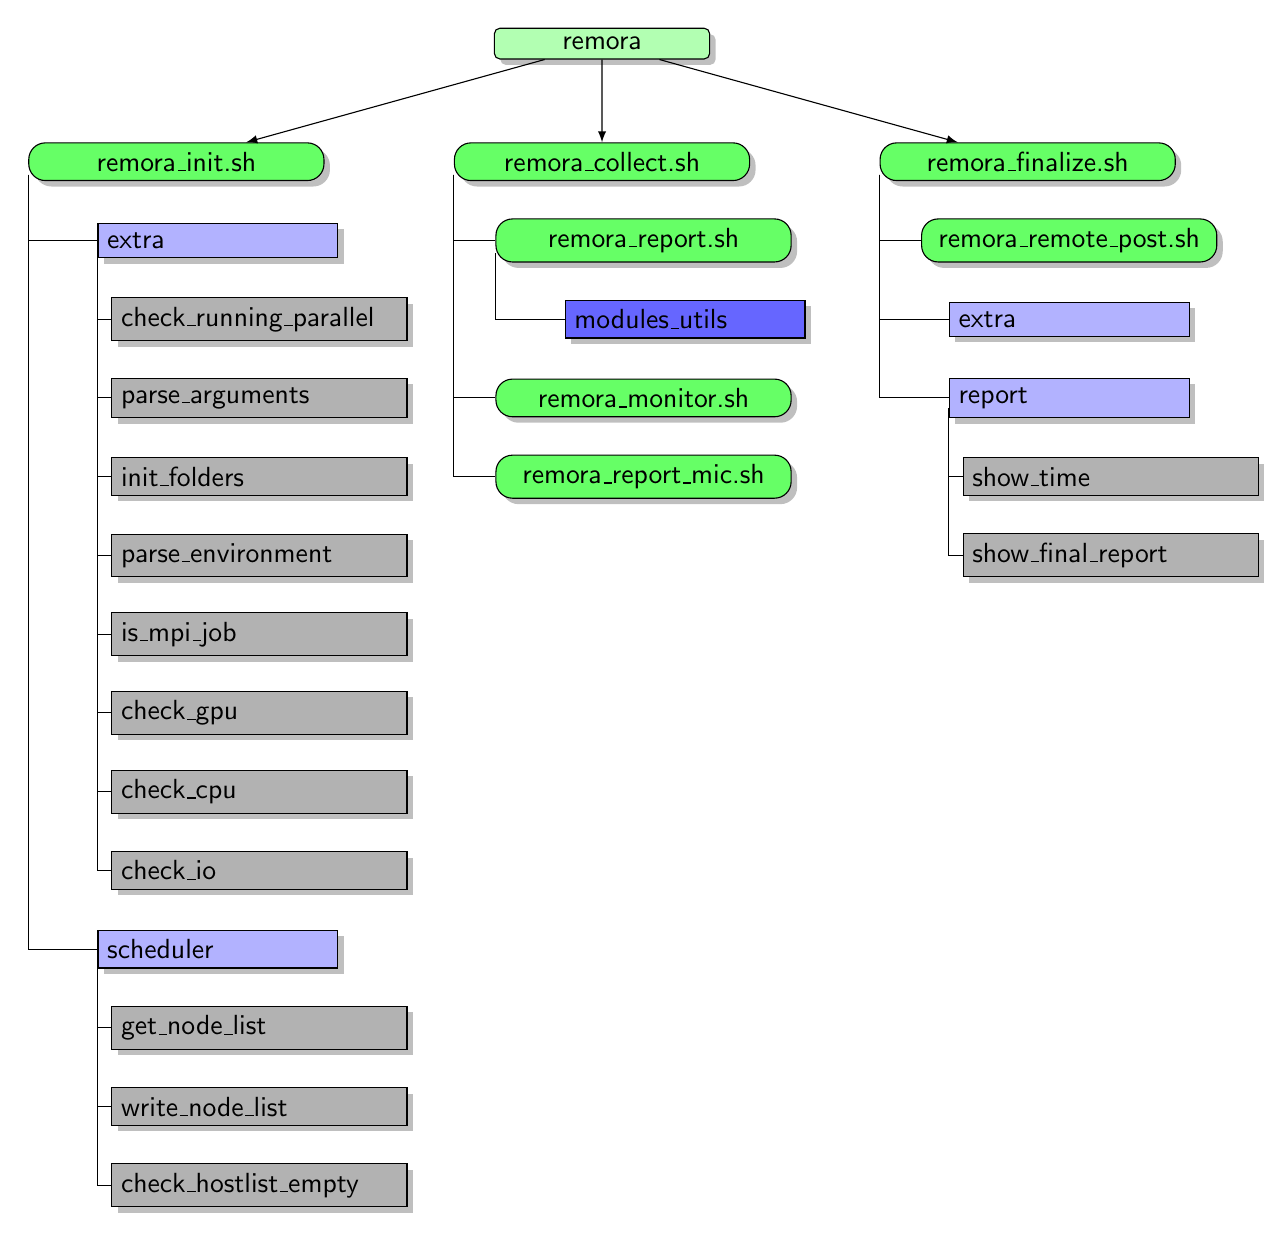
\begin{tikzpicture}[level 1/.style={sibling distance=40mm},edge from parent/.style={->,draw},>=latex]

% scripts are level 2, aux is level 3, modules is level 4, bash funcs are level 5

\node[root] { remora }
  child {node[level 2, xshift=-40pt] (c1) {remora\_init.sh} }
  child {node[level 2] (c2) {remora\_collect.sh} }
  child {node[level 2, xshift=40pt] (c3) {remora\_finalize.sh} };
  
\node [level 3, below of = c1, xshift=15pt] (c11) {extra};
\node [level 5, below of = c11, xshift=15pt] (c111) {check\_running\_parallel};
\node [level 5, below of = c111] (c112) {parse\_arguments};
\node [level 5, below of = c112] (c113) {init\_folders};
\node [level 5, below of = c113] (c114) {parse\_environment};
\node [level 5, below of = c114] (c115) {is\_mpi\_job};
\node [level 5, below of = c115] (c116) {check\_gpu};
\node [level 5, below of = c116] (c117) {check\_cpu};
\node [level 5, below of = c117] (c118) {check\_io};

\node [level 3, below of = c118, xshift=-15pt] (c12) {scheduler};
\node [level 5, below of = c12, xshift=15pt] (c121) {get\_node\_list};
\node [level 5, below of = c121] (c122) {write\_node\_list};
\node [level 5, below of = c122] (c123) {check\_hostlist\_empty};

\node [level 2, below of = c2, xshift=15pt] (c21) {remora\_report.sh};
\node [level 4, below of = c21, xshift=15pt] (c211) {modules\_utils};
\node [level 2, below of = c211, xshift=-15pt] (c22) {remora\_monitor.sh};
\node [level 2, below of = c22] (c23) {remora\_report\_mic.sh};

\node [level 2, below of = c3, xshift=15pt] (c31) {remora\_remote\_post.sh};
\node [level 3, below of = c31] (c32) {extra};
\node [level 3, below of = c32] (c33) {report};
\node [level 5, below of = c33, xshift=15pt] (c331) {show\_time};
\node [level 5, below of = c331] (c332) {show\_final\_report};


\foreach \value in {1,2}
  \draw[-] (c1.185) |- (c1\value.west);
\foreach \value in {1,2,3}
  \draw[-] (c2.185) |- (c2\value.west);
\foreach \value in {1,2,3}
  \draw[-] (c3.185) |- (c3\value.west);
  
\foreach \value in {1,...,8}
  \draw[-] (c11.185) |- (c11\value.west);
\foreach \value in {1,2,3}
  \draw[-] (c12.185) |- (c12\value.west);
\foreach \value in {1}
  \draw[-] (c21.185) |- (c21\value.west);
\foreach \value in {1,2}
  \draw[-] (c33.185) |- (c33\value.west);
   
\end{tikzpicture}

\FloatBarrier
\chapter{Expanding REMORA's Functionality}\label{expand-remora}

Since version 1.6.0, REMORA allows system administrators to easily change the functionality provided by REMORA and extend its capabilities. The configuration file \verb+src\config\modules+ defines the modules used by REMORA. Each module provides a specific capability in terms of data collection. By default, these are the modules available in REMORA:

\begin{itemize}
\item cpu
\item memory
\item numa
\item lustre
\item lnet
\item dvs
\item ib
\item gpu
\item network
\end{itemize}

These modules are currently specified in the configuration file. At runtime, REMORA will read this file and execute all the modules listed on it.

We are trying to provide modules that required no elevated privileges in the system. If you are willing to run remora as root, or using a setuid binary then you can easily extend it to support GPFS data collection.

\IntroBox{If you are installing REMORA system-wide, you can modify the configuration file before installing it. If you have REMORA installed in your user account, you can modify this file at any time.}

\section{Structure of Modules}

All the modules are located in the \verb+src/modules/+ folder. They are all bash scripts that have to implement, at least, the following functions:

\begin{itemize}
	\item \texttt{init\_module\_modulename()}: this function is called only once to initialize the environment or files that are required by each specific module.
	\item \texttt{collect\_data\_modulename()}: main function of the module. This is the function called each \texttt{REMORA\_PERIOD} seconds. Depending on the module, different statistics will be collected in this function. This function can include some postprocessing.
	\item \texttt{process\_data\_modulename()}: currently unused.
	\item \texttt{monitor\_data\_modulename()}: real time post-processing of captured data
	\item \texttt{finalize\_module\_modulename()}: this function is also called only once, when the application of interest has finished. Any heavy postprocessing method can go in this function.
\end{itemize}

All these functions take two, and only two, arguments:
\begin{itemize}
	\item Name of the compute node where the function is going to run.
	\item Full path to the output folder.
\end{itemize}

The \texttt{modulename} is exactly the same name specified in the configuration file and also the filename of the bash script. This means that, if we have a module called \texttt{cpu} in the configuration file, there will be a file named \texttt{cpu} in the modules folder. And, inside that file, the required functions will be called:

\begin{itemize}
	\item \texttt{init\_module\_cpu()}
	\item \texttt{collect\_data\_cpu()}
	\item \texttt{process\_data\_cpu()}
	\item \texttt{monitor\_data\_cpu()}
	\item \texttt{finalize\_module\_cpu()}
\end{itemize}


\section{Creating a New Module}

REMORA has been designed so that expanding its functionality is very simple. If you want to create a new module, let's call it \texttt{newmodule}, you will need to follow these steps:

\begin{enumerate}
	\item Add a new line to the configuration line with the string \texttt{newmodule}.
	\item Create a new file in the \verb+src/modules+ folder called \texttt{newmodule}.
	\item Inside this new file, define the following functions:
		\begin{itemize}
			\item \texttt{init\_module\_newmodule()}
			\item \texttt{collect\_data\_newmodule()}
			\item \texttt{process\_data\_newmodule()}
			\item \texttt{monitor\_data\_newmodule()}
			\item \texttt{finalize\_module\_newmodule()}
		\end{itemize}
	\item Implement the functionality that \texttt{newmodule} requires in those functions.
\end{enumerate}

At runtime, REMORA will find the new module specified in the configuration file and call the different functions at runtime.

\IntroBox{It is very important to make sure that all the functions contain exactly the same name of the module included in the configuration file and used as filename for the module.}

It is possible to use an existing system wide installation to check new modules. Two environment variables can be used:
\begin{itemize}
        \item \texttt{REMORA\_CONFIG\_PATH}: path to the configuration file (named config). If defined, REMORA will only use the modules specified on that file, not the previously existing ones.
        \item \texttt{REMORA\_MODULE\_PATH}: path to the modules. By default, REMORA looks in \texttt{REMORA\_BIN/modules}, but users can create their own modules and store them somewhere else. If defined, system modules will not be used.
\end{itemize}

\FloatBarrier
\addcontentsline{toc}{section}{\bf References}
\begin{thebibliography}{00}

\bibitem{remora} C. Rosales, A. G\'{o}mez-Iglesias, A. Predoehl. ``REMORA: a Resource Monitoring Tool for Everyone''. HUST2015 November 15-20, 2015, Austin, TX, USA. DOI: \href{http://dx.doi.org/10.1145/2834996.2834999}{10.1145/2834996.2834999}


\end{thebibliography}

\end{document}
